\section{混入(Mixins)}
Mixins是一种小型类,用于向其他类添加功能。若读过关于Mixins的文章,会发现在C++中使用奇异递归模板模式来实现Mxins,但这是一个不正确的说法。CRTP有助于实现与Mixins类似的目标,但它们是不同的技术。Mixins的关键在于,向类添加功能,而不是作为类的基类。而作为基类,是CRTP模式的关键。相反,Mixins应该从它们添加功能的类继承,属于逆CRTP。

还记得前面关于骑士和法师的例子吗?可以使用step\_forth和step\_back成员函数来回移动。骑士和法师的职业是从movable\_unit类模板派生出来的,该模板添加了advance和retreat的功能,这使得单位可以向前或向后移动几步。同样的例子可以以相反的顺序使用Mixins来实现。以下是具体实现:

\begin{cpp}
struct knight
{
	void step_forth()
	{
		std::cout << "knight moves forward\n";
	}
	void step_back()
	{
		std::cout << "knight moves back\n";
	}
};
struct mage
{
	void step_forth()
	{
		std::cout << "mage moves forward\n";
	}

	void step_back()
	{
		std::cout << "mage moves back\n";
	}
};

template <typename T>
struct movable_unit : T
{
	void advance(size_t steps)
	{
		while (steps--)
			T::step_forth();
	}

	void retreat(size_t steps)
	{
		while (steps--)
			T::step_back();
	}
};
\end{cpp}

knight和mage现在是没有基类的职业,都提供了step\_forth和step\_back成员函数,就像之前实现的CRTP模式。现在,movable\_unit类模板是从这些类中派生出来的,并定义了advance和retreat函数,并在循环中调用了step\_forth和step\_back。可以这样使用:

\begin{cpp}
movable_unit<knight> k;
k.advance(3);
k.retreat(2);

movable_unit<mage> m;
m.advance(5);
m.retreat(3);
\end{cpp}

这与使用CRTP模式非常相似,除了创建的实例是movable\_unit<knight>和movable\_unit<mage>,而不是knight和mage。两种模式的比较如下图所示(左边是CRTP,右边是Mixins):

\begin{center}
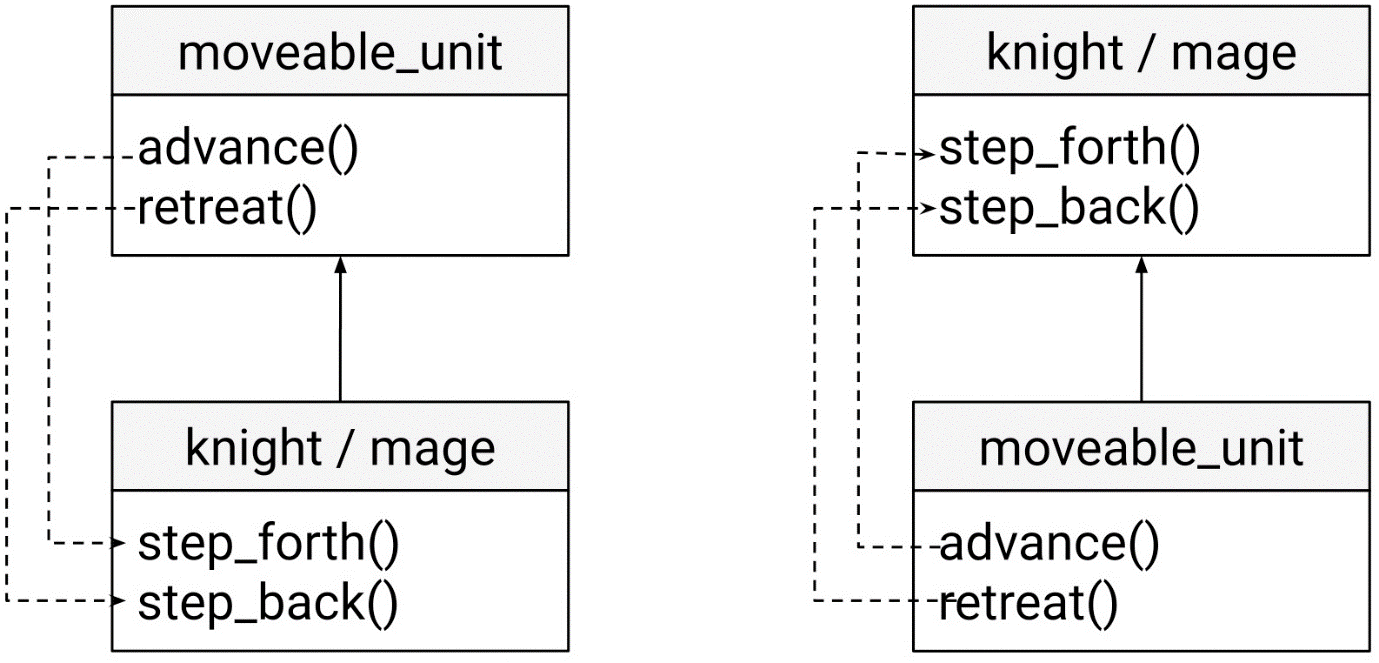
\includegraphics[width=0.7\textwidth]{images/1.png}\\
图7.1:CRTP和Mixins模式的比较
\end{center}

可以结合使用Mixins实现的静态多态,与使用接口和虚函数实现的动态多态。这里将通过一个关于战斗的游戏单位来说明这一点。我们之前在讨论CRTP时举过一个例子,其中knight和mage职业都有一个叫做attack的成员函数。

假设想要定义多种攻击风格。例如,每个游戏单位可以使用侵略性或中等攻击风格。所以这意味着四种组合:侵略性和中等骑士,侵略性和中等法师。另一方面,骑士和法师都可能是喜欢独自战斗的孤独战士,或者是总是与其他单位一起战斗的团队成员。

我们可以有单独的好斗骑士和温和骑士,也可以有团队合作的好斗骑士和温和骑士,这同样适用于法师。组合的数量增长了很多,Mixins是一个很好的方式来提供这种额外的功能,而不扩大knight和mage的职业。最后,我们希望能够在运行时多态地处理所有这些。现在,来看看怎么做。

首先,可以定义好斗和温和的战斗风格。简单实现如下所示:

\begin{cpp}
struct aggressive_style
{
	void fight()
	{
		std::cout << "attack! attack attack!\n";
	}
};

struct moderate_style
{
	void fight()
	{
		std::cout << "attack then defend\n";
	}
};
\end{cpp}

接下来,将Mixins定义为能够独自或在团队中战斗的需求。这些类是模板,由模板参数派生:

\begin{cpp}
template <typename T>
struct lone_warrior : T
{
	void fight()
	{
		std::cout << "fighting alone.";
		T::fight();
	}
};
template <typename T>
struct team_warrior : T
{
	void fight()
	{
		std::cout << "fighting with a team.";
		T::fight();
	}
};
\end{cpp}

最后,需要定义knight和mage职业,这些本身就是战斗风格的Mixins。为了能够在运行时多态地进行处理,我们从game\_unit类中派生出它们,这个类包含一个叫做attack的纯虚方法:

\begin{cpp}
struct game_unit
{
	virtual void attack() = 0;
	virtual ~game_unit() = default;
};

template <typename T>
struct knight : T, game_unit
{
	void attack()
	{
		std::cout << "draw sword.";
		T::fight();
	}
};

template <typename T>
struct mage : T, game_unit
{
	void attack()
	{
		std::cout << "spell magic curse.";
		T::fight();
	}
};
\end{cpp}

knight和mage的attack成员函数使用了T::fight方法,aggresive\_style和moderate\_style类,以及lone\_warrior和team\_warrior混合类都提供了这样的成员函数。所以,可以进行以下组合:

\begin{cpp}
std::vector<std::unique_ptr<game_unit>> units;

units.emplace_back(new knight<aggressive_style>());
units.emplace_back(new knight<moderate_style>());
units.emplace_back(new mage<aggressive_style>());
units.emplace_back(new mage<moderate_style>());
units.emplace_back(
	new knight<lone_warrior<aggressive_style>>());
units.emplace_back(
	new knight<lone_warrior<moderate_style>>());
units.emplace_back(
	new knight<team_warrior<aggressive_style>>());
units.emplace_back(
	new knight<team_warrior<moderate_style>>());
units.emplace_back(
	new mage<lone_warrior<aggressive_style>>());
units.emplace_back(
	new mage<lone_warrior<moderate_style>>());
units.emplace_back(
	new mage<team_warrior<aggressive_style>>());
units.emplace_back(
	new mage<team_warrior<moderate_style>>());

for (auto& u : units)
	u->attack();
\end{cpp}

这里总共定义了12种组合,而这一切只需要6个类就能实现。这显示了Mixins如何添加功能,同时将代码的复杂性保持在较低的水平。若运行代码,会得到以下输出:

\begin{shell}
draw sword.attack! attack attack!
draw sword.attack then defend
spell magic curse.attack! attack attack!
spell magic curse.attack then defend
draw sword.fighting alone.attack! attack attack!
draw sword.fighting alone.attack then defend
draw sword.fighting with a team.attack! attack attack!
draw sword.fighting with a team.attack then defend
spell magic curse.fighting alone.attack! attack attack!
spell magic curse.fighting alone.attack then defend
spell magic curse.fighting with a team.attack! attack attack!
spell magic curse.fighting with a team.attack then defend
\end{shell}

这里看到了两种模式,CRTP和Mixins,都旨在向其他类添加额外的(公共)功能。尽管看起来很相似,但它们的结构不同,不应该混淆。利用不相关类型的通用功能的另一种技术称为类型擦除,我们将在下一节进行讨论。



































